% NIH Grant Proposal for the Specific Aims and Research Plan Sections
%----------------------------------------------------------------------------------------
%	PACKAGES AND OTHER DOCUMENT CONFIGURATIONS
%----------------------------------------------------------------------------------------

\documentclass[11pt,notitlepage]{article}

% A note on fonts: As of 2013, NIH allows Georgia, Arial, Helvetica, and Palatino Linotype. LaTeX doesn't have Georgia or Arial built in; you can try to come up with your own solution if you wish to use those fonts. Here, Palatino & Helvetica are available, leave the font you want to use uncommented while commenting out the other one.

\usepackage[super]{natbib}
\usepackage{palatino} % Palatino font
%\usepackage{helvet} % Helvetica font
\renewcommand*\familydefault{\sfdefault} % Use the sans serif version of the font
\usepackage[T1]{fontenc}
\linespread{1.05} % A little extra line spread is better for the Palatino font
\usepackage{hyperref} % to allow hyperlinks to websites on the internet
\usepackage[hypcap]{caption} % to point to the top of the image
\usepackage{lipsum} % Used for inserting dummy 'Lorem ipsum' text into the template
\usepackage{amsfonts, amsmath, amsthm, amssymb} % For math fonts, symbols and environments
\usepackage{graphicx} % Required for including images
\usepackage{booktabs} % Top and bottom rules for tables
\usepackage{wrapfig} % Allows in-line images
%\usepackage[labelfont=\small]{caption} % Make figure numbering in captions bold
\usepackage[top=0.6in,bottom=0.6in,left=0.6in,right=0.6in]{geometry} % Reduce the size of the margin

\usepackage{booktabs}
\usepackage{graphicx}
\usepackage[table,xcdraw]{xcolor}
\pagestyle{empty} % Remove page numbers
%\let\oldtabular\tabular 
%\renewcommand{\tabular}{\large\oldtabular}

\hyphenation{ionto-pho-re-tic iso-tro-pic fortran} % Specifies custom hyphenation points for words or words that shouldn't be hyphenated at all

  % to reduce white space between SECTIONS
\usepackage[compact]{titlesec}
\titlespacing{\part}{0pt}{*0pt}{*0pt}
\titlespacing{\section}{0pt}{*0}{*0}
\titlespacing{\subsection}{0pt}{*0}{*0}
\titlespacing{\subsubsection}{0pt}{*0}{*0}

% Reduce whitespace arount lists
\usepackage{mdwlist}

%\usepackage[compact]{titlesec}
%\titlespacing{\part}{-200pt}{-100pt}{-200pt}
%\titlespacing{\section}{0pt}{0pt}{0pt}
%\titlespacing{\subsection}{0pt}{*0}{*0}
%\titlespacing{\subsubsection}{-2pt}{*0}{*0}
%\titlespacing{\subparagraph}{-5pt}{*0}{*0}
%\titlespacing*{\subparagraph} {\parindent}{1ex plus 1ex minus .2ex}{0.5em}

  
  % to reduce white space between PARAGRAPHS
%\setlength{\parskip}{-2pt}
% \setlength{\parsep}{-2pt}

  % additional parameters
\setlength{\headsep}{20pt}
%\setlength{\topskip}{0pt}
%\setlength{\topmargin}{0pt}
%\setlength{\topsep}{0pt}
\setlength{\partopsep}{-2pt}
%\setlength{\parindent}{1cm}

% to reduce white space around figures
% \setlength{\textfloatsep}{0pt plus 0pt minus 0pt}

% Set graphics path to tell latex where to look for images
%\graphicspath{ {C:/Users/Micheal/Dropbox/Professional/KL2/BigDataR01/ConceptGraphics/} }

\begin{document}
\part*{Specific Aims}
National health databases and electronic health records (EHR) are inherently 
clustered by procedure, provider, service, institution and geography. Often 
neglected, this rich spatial and temporal organization is most realistically 
captured in hierarchical statistical models with cluster-specific parameters, but 
estimating such models is still computationally difficult for traditional software. 
We propose to further develop capabilities of \textit{Stan}, a novel, probabilistic 
programming language, to make advanced hierarchical modeling more readily accessible 
to data scientists for medical outcomes research. 

\paragraph*{Flexibility and robustness of hierarchical modeling could 
transform EHR based outcomes research.} Consider surgery as an 
illustrative example. Patients in the same hospital undergoing the 
same surgical intervention by the same team will show similar clinical 
trajectories and responses. We are interested in investigating
differences in therapeutic effects or to predict poor outcomes in order to prevent 
them. (1) Estimating individual intercept-shifts for each provider and procedure
can help to control for potentially confounding differences 
in quality of care by different teams. (2) Spatial clustering of adherence 
behavior, e.g., by different services, can be represented by multilevel modeling. 
(3) Partial pooling can improve parameter estimates, especially in subgroups with sparse data.
For example, prediction of adverse health outcomes can be 
improved by exploiting the implied correlations between different but related subsets of data. 
Failure to account for the highly structured and correlated nature of health care delivery may lead 
to incorrect statistical inferences, poor predictions, and adverse health consequences. 
Realistic modeling of the heterogeneity in  care delivered may help to identify reasons for variance in outcomes.

\paragraph*{Classical approaches and software packages often lack flexibility 
for hierarchical modeling.} Available software limits the types of 
hierarchical models that can be estimated because their algorithms are more likely 
to run into convergenc problems or other errors with more complicated hierarchical models.
In contrast, \textit{Stan} is a flexible, general-purpose modeling language that has 
facilitated hierarchical modeling in biostatistics, epidemiology, public health 
political science, and pharmacokinetic modeling. Nevertheless, \textit{Stan's} novel 
implementation of Hamiltonian Monte Carlo makes it feasible to estimate 
even advanced and nontraditional statistical models. \textit{Stan's} development has been funded 
by the NSF, DoD, and other organizations. \textit{Stan} and its interfaces (from \textit{Python, Julia, R}, etc.) 
are open source and platforms independent. 

\paragraph*{Robust, efficient, expressive and accessible software promotes Big 
Data outcomes research.} At present, it still takes a computationally 
sophisticated statistician to write a hierarchical model from scratch, to transform 
the data to facilitate convergence of the algorithm, and to correctly index the group 
indicators in a hierarchical model. We lack intuitive diagnostic, visual and exploratory 
tools to recognize when a model is logically flawed or fails to fit the data empirically. 
We propose to further enhance sophisticated hierarchical model 
building for clinical and health services research by developing and expanding 
\textit{Stan} and its ecosystem of \textit{Stan}-related software to 
incorporate interactive and intuitive statistical tools to facilitate principled model 
checking and respecification.

\noindent \textbf{Specific aims}
\paragraph*{Aim 1:} To advance and expand our simple and user-friendly software 
\textit{rstanarm} for the open-source statistical environment \textit{R} 
in collaboration with applied clinical data scientists and biostatisticians. To 
make advanced hierarchical modeling of EMR computationally efficient and readily 
accessible to average clinical data scientists with a simple function call for a 
representative class of hierarchical models.

\paragraph*{Aim 2:} To harden and further develop \textit{shinystan}, our 
interactive web application to analyze and visually explore the output of hierarchical 
models and to develop novel principled diagnostics to identify and troubleshoot
computational and empirical problems with advanced hierarchical models.

\paragraph*{Aim 3:} To explicate, document and disseminate realistic hierarchical 
modeling and its advanced computational implementation to the 
clinical data science community with hands on use cases, workshops, journal articles, and 
online tutorials. To solicit the data scientist community feedback, engage new 
software developers and to incorporate improvements to our software through 
online user and developer groups.

\part*{Research Strategy}

\part*{Significance}

\section*{The nested structure of health care delivery and electronic health data}
Clinical data scientists are faced with an abundance of useful electronic health data, 
but limitations of existing statistical inference tools constrain the scientific 
hypotheses they can explore. Electronic health related data sets 
are growing rapidly in the number of units of observation and 
variables observed. This growth implies that we can investigate increasingly fine-grained 
models. Whereas before we were limited to models of the mean structure and effect, we 
now want to our models to account for clinical heterogeneity.

\subsection*{The National Anesthesia Clinical Outcomes Registry}
Below we illustrate the clustered, nested data structure of contemporary health 
care delivery and electronic health data capture with the example of the 
National Anesthesia Clinical Outcomes Registry (NACOR). NACOR is maintained by the 
Anesthesia Quality Institute and funded by the American Society of 
Anesthesiologists, and we will utilize NACOR as a use case for dissemination in 
workshops for perioperative data scientists.

\subsection*{Perioperative health care delivery and data capture are nested and clustered.}
Anesthesia is an illustrative case of the how health care is increasingly 
electronically documented, which facilitates the continuous collection of 
physiological data and therapeutic interventions during critical periods. In order to 
support building, this electronically captured data 
is jointed with surgical and anesthesia procedure codes International 
Classification of Disease (ICD) codes, provider identifiers, patient perioperative 
risk, outcome and provider compliance assessment. Participating institutions upload 
this comprehensive file from their anesthesia information management systems 
(AIMS) directly to NACOR. NACOR contains at present over 30 million individual 
electronic records of anesthesia care provided and, like similar databases, is 
growing rapidly. This data set invites health services and outcomes research, 
but (as pointed out in the letter of support by Dr. Dutton, last director or 
NACOR and Dr. Kheterpal director of MPOG, the other large perioperative EHR 
database) their exploitation is limited by the lack of accessible software to investigate 
important scientific questions with realistic hierarchical models.

\subsection*{Outcomes and care delivered depend on procedure, providers and patient characteristics.} 

\begin{wrapfigure}{l}{0.4\textwidth} 
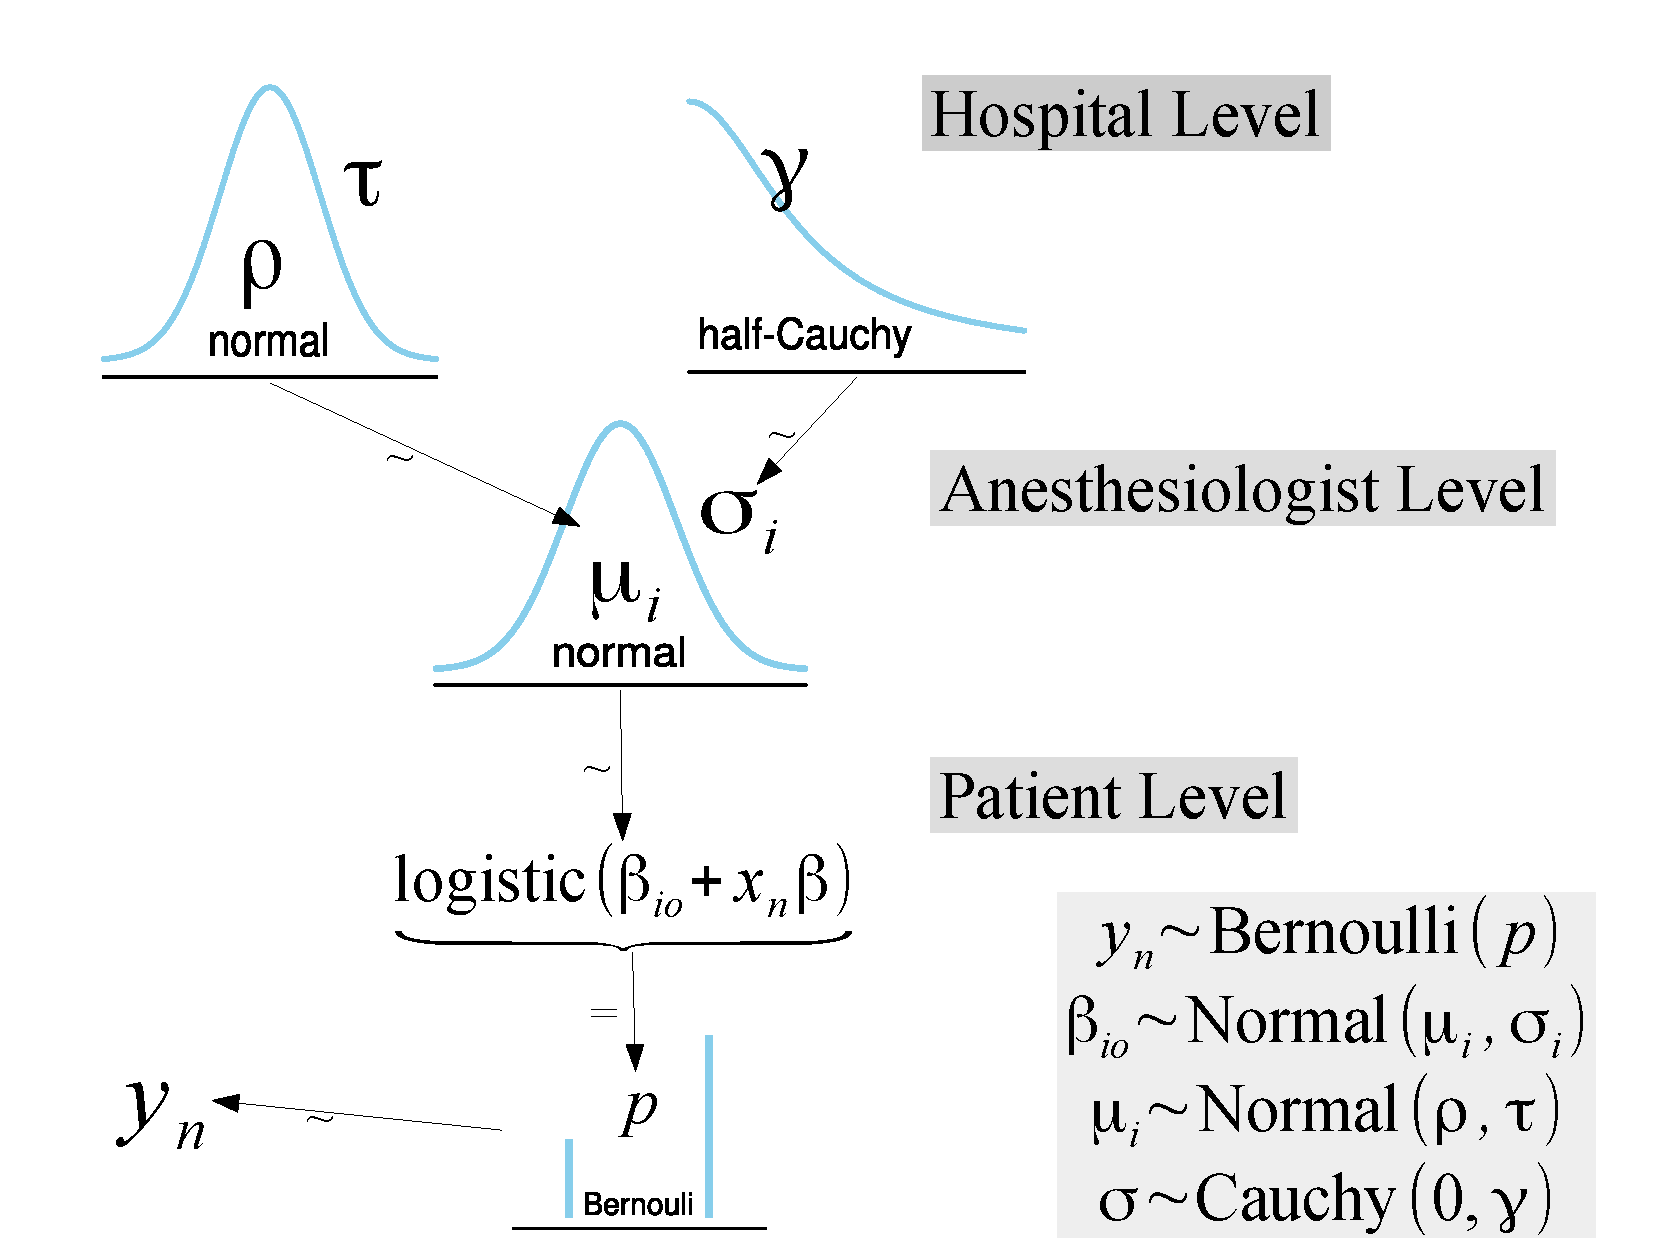
\includegraphics[width=0.4\textwidth]{Figures/DistrogramNACOR.pdf} 
\caption{Hierarchical structure of health care delivered in the perioperative setting.}
\label{fig:NACOR}
\end{wrapfigure}

Figure \ref{fig:NACOR} explains the hierarchical structure of health care delivery with our model on anesthesia quality 
using NACOR data. The (dichotomous) outcome of particular anesthetic for a given individual, (e.g., postoperative nausea), 
will depend on the surgical procedure the patient is undergoing and under which service, but also depends on the local 
institutional culture and indeed the individual anesthesia provider and his or her qualifications and preferences \cite{AndreaeWhite2015}. 
Outcome $y_n$ for the $n$th patient is a Boolean indicator to be predicted by a logistic regression. We allow the patient-specific
intercept $\beta_{oi}$ to vary according to the $i$th anesthesiology provider caring for the patient. The provider level mean 
$\mu_i$ and within-provider variance $\sigma_i$ vary by hospital. $x_n$ is a vector of patient level predictors, and $\beta$ is a vector 
of regression coefficients.  

We seek to further illustrate the nested structure of outcome data in health care with two examples from labor analgesia and spine surgery: 
Anesthesiologists may feel more or less inclined or competent to offer regional anesthesia techniques. Provision of epidural labor 
anesthesia varies widely across the nation and within an institution and is predicted by socioeconomic and racial patient characteristics 
\cite{Rust2004,Glance2007}. There is substantially less bleeding, on average, during spine surgery when performed by a neurosurgeons than by an 
orthopedic surgeon. However, a particularly gifted orthopedic surgeon may outperform the average neurosurgeon with regards to surgical 
blood loss.

\section*{Hierarchical models capture contemporary health care practice realistically}
Hierarchical modeling could transform electronic health records based outcomes research, because the rich spatial and temporal 
organization of electronic health records is most realistically captured in hierarchical statistical models. However, efficient model 
fit and computational implementation are still difficult.  Additional depth of data (simply more units of observation) would increase 
the precision of estimates and generally make our clinical data analysis easier. However, there is also more breadth to the data: 
more subgroups, locations, provider or time granularity than is currently being modeled. There are more partial, incomplete and noisy 
measurements that cannot easily be incorporated into standard models and more related studies that are available for meta-analysis
\cite{Andreae2015,Andreae2012}.

\subsection*{Modeling the multifaceted correlations in EHR is reflecting actual clinical practice}
To realistically model the multifaceted correlations seen in actual clinical 
practice, we specify a regression model that predicts anesthesia quality in the NACOR database
with regression coefficients that vary by provider, where providers are again nested by service or by hospital
\cite{AndreaeWhite2015}. We needed to adjust for the surgical procedure type as well, and there are thousands 
of different surgical procedures performed in the NACOR data. The number of parameters to estimate grows very quickly 
and so do the potential interactions. Even with very large data sets, the  
size of each subgroup will shrink rapidly and estimates using least squares or 
maximum likelihood have little statistical justification and often are too noisy to be useful. 
One solution lies in hierarchical modeling, where we estimate hyper-parameters 
and hyper-hyper-parameters (Figure~ \ref{fig:NACOR}), which allows lower 
level parameters to vary across groups \cite{Bafumi_Gelman_2007}. 
In hierarchical models, we take advantage of shrinkage; in other words we 
can borrow strength from larger groups to improve estimates for smaller 
subgroups as explained below \cite{ParkGelman2004bayesian}.

\subsection*{Hierarchical models provide efficient inferences with partial pooling}
Inference based on partial pooling outperforms (a) the No-pooling and (b) the 
complete-pooling approaches, as can be shown mathematically \cite{Efron_1975} 
or via cross-validation \cite{Gelman-Hill_2014}: By trading an increase in bias 
for a reduction in variance, hierarchical modeling can reducing the mean square error.  

(a) Using the No-pooling approach, we would separately estimate the model for each 
subset of interest. Howerver, there are far too many sub-classifications, 
(e.g., one model for each type of surgery) and thus the sample is too small in any given 
subgroup to make useful inferences, despite the richness of the EMR data.

(b) Employing complete pooling or structural modeling constitutes the other extreme 
of the spectrum, but the implied equality constraints on the coefficients in different 
groups may lead to bias. Ignoring the obvious known differences in the data --- such 
as between patients undergoing tracheotomy versus cesarean section --- glosses
over this granular detail.

We choose the middle ground: for our richly organized NACOR data set, inference 
using partial pooling or hierarchical modeling is especially effective because 
the estimate of each individual parameter is simultaneously informed by data from 
all the other patients in our cohort, which especially improves prediction for 
subgroups with sparse data. \cite{Gelman2009}. Efron explained this apparent 
paradox well to non-statisticians in the 
\href{http://www.nature.com/scientificamerican/journal/v236/n5/pdf/
scientificamerican0577-119.pdf}{Scientific American}
\cite{Stein_paradox_Scientific_American}. 
Our co-investigator, Dr. Hall, applied this recently to seizure prediction \cite{Hall2009a}. 

\subsubsection*{Borrowing strength is beneficial even in very large data sets}
In summary, the geographic, spatial and other above outlined heterogeneities 
in actual health care provided can undermine precision or accuracy even for 
extremely large clinical data sets. Partial pooling can improve inferences and prediction
by borrowing strength from different but related instances
\cite{Tukey1963borrowing,Jones1986collected}. 

\section*{Meta-analysis: hierarchical modeling for data driven outcomes research}
Meta-analysis, the synthesis of clinical outcome data to support evidence based decision making, is another 
example of hierarchical modeling where current software and classical modeling approaches limit progress in 
data driven outcomes research \cite{Andreae2015}. Clinicians are familiar with systematic reviews and 
meta-analysis \cite{Sackett1996}. Evidence synthesis (a more accurate term than meta-analysis) is a powerful tool 
to pool clinical trials to guide evidence based clinical care \cite{Ashby2000}. Rigorous evidence synthesis is 
considered the highest level of evidence to support clinical decision making \cite{Cook1997}. 

\subsection*{Variance in study design and outcome reporting hamper evidence synthesis}
However, studies on perioperative outcomes tend to vary in design and reported outcomes\cite{Andreae2013}, making 
evidence synthesis challenging with classical frequentist statistical models \cite{Spiegelhalter_11134920}, (see 
letter of support by Dr. Sacks). Different study designs can make it difficult to perform meta-analysis or meta-regression 
with classical methods and standard systematic review software \cite{Deeks2011chapter}. Classical meta-analysis may also 
underestimate the between-study-variability for small numbers of trials \cite{Song2012,Cornell2014,Andreae2015}. 
\textit{Classical} meta-analysis is an example of data with a \textit{single} level of hierarchical grouping: patients' 
outcomes are grouped within clinical trials \cite{egger2008systematic}. There are however several constraints and limitations 
with this classical approach to meta-analysis that can be overcome with more sophisticated hierarchical modeling  
\cite{Andreae2015,Thompson2002,Abroug2011}.

\subsubsection*{Hierarchical models integrate all available data for evidence synthesis}

\begin{wrapfigure}{l}{0.35\textwidth} 
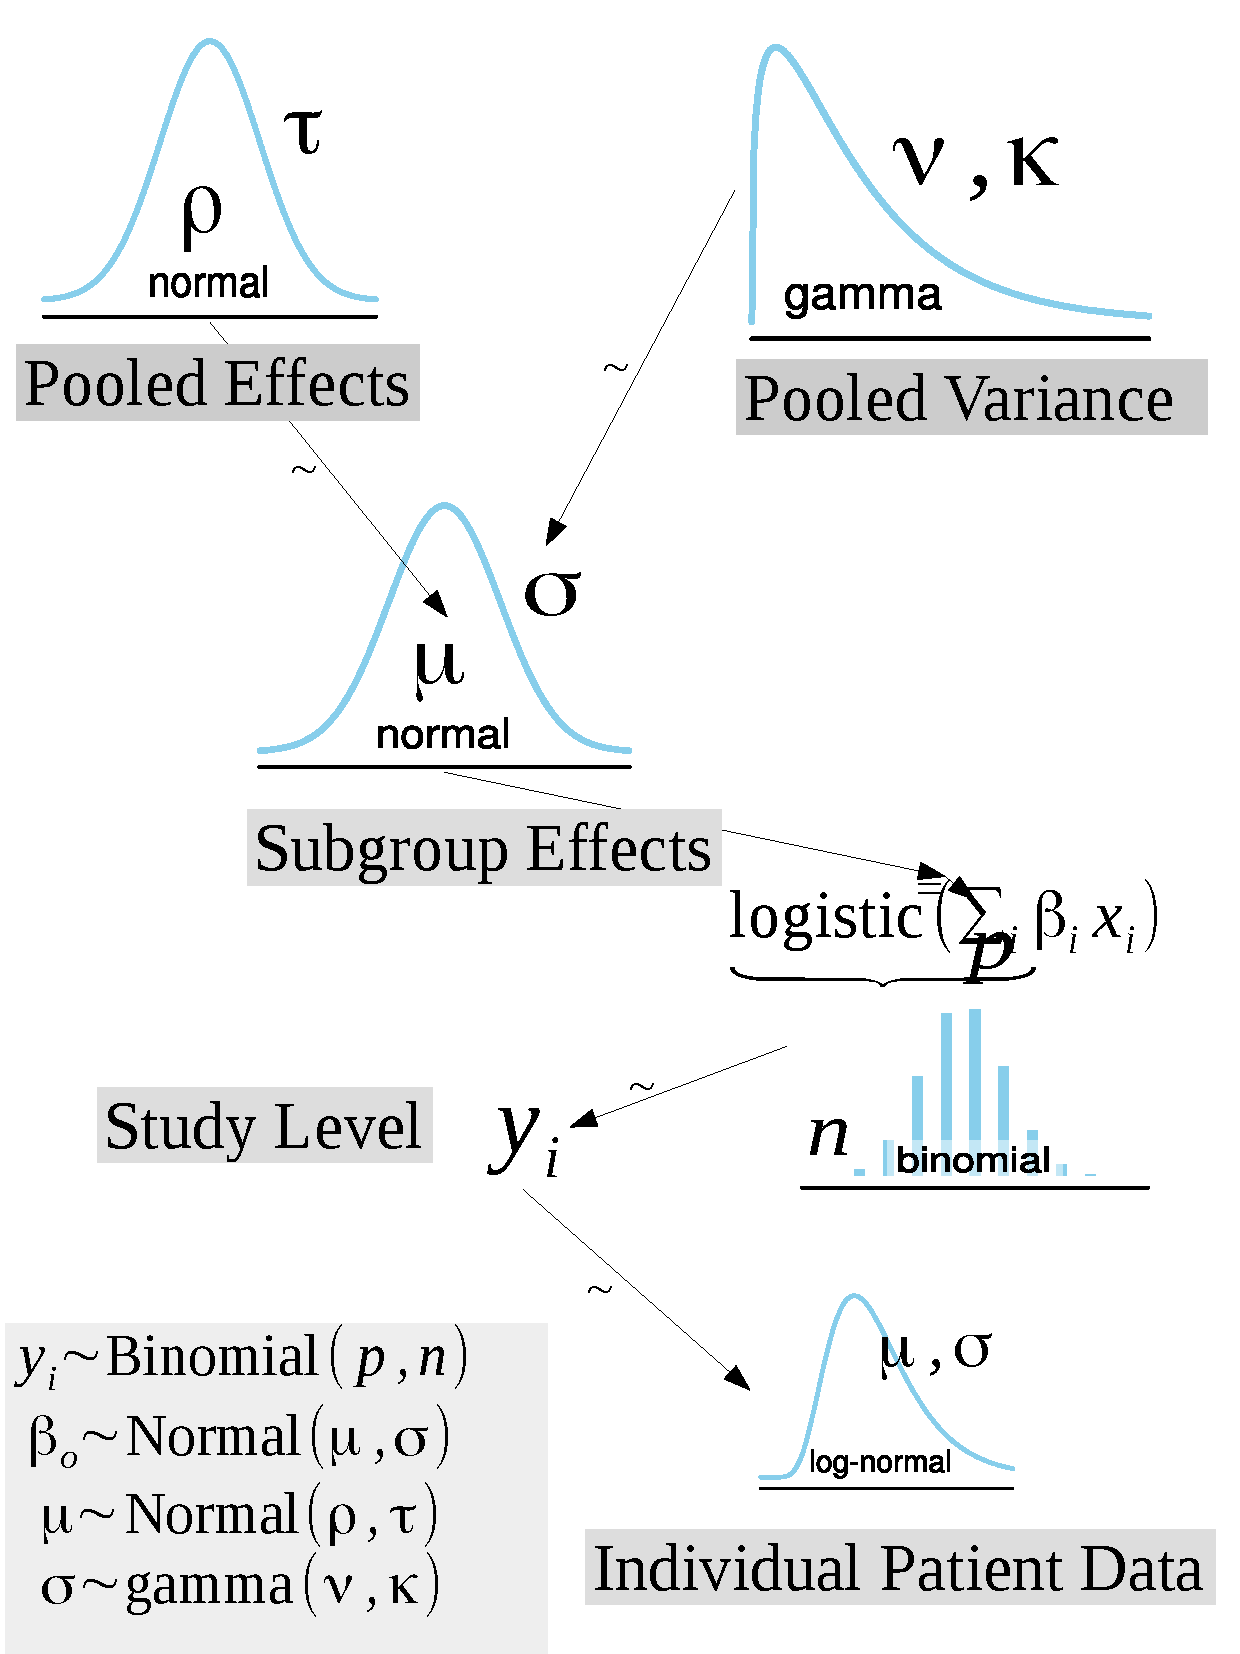
\includegraphics[width=0.35\textwidth]{Figures/DistrogramMultiLevelMetaAnalysis.pdf} 
\caption{Multi-level meta-analysis.}
\label{fig:MetaAnalysis}
\end{wrapfigure}

Trial or population characteristics may introduce another level of grouping, for example pooling long term outcomes 
after regional anesthesia by surgical intervention \cite{Andreae2013,Abroug2011}. Trials may observe outcomes at several 
sequential follow-up visit, leading to repeated (correlated) observations grouped by patient that are then grouped by trial 
in the meta-analysis.  We build a multilevel hierarchical model to pool individual patient data with continuous and 
dichotomous aggregate study level data, clustered at the study level by followup interval and at the study level by surgical 
intervention performed (Figure \ref{fig:MetaAnalysis}). Besides the three levels of hierarchical modeling just outlined 
(follow-up observations grouped by patient, patients grouped withing trials, trials within population), additional groupings 
or hierarchical levels concern exposure dose, as meta-regression of effect dose dependence may explain substantial between-study 
variance in outcomes reported to reconcile study findings \cite{Andreae2015}. Evidence synthesis may seek to integrate continuous 
with dichotomous outcome measures \cite{AndreaeJohnsonAbstract2013}, because to be valid meta-analysis must integrate \textit{all} 
available data sources \cite{Deeks2011chapter}. However, short of having access to all individual patient data, the integration of 
dichotomous outcomes with continuous outcomes is challenging with classical methods\cite{Andreae2015}, especially as often insufficient 
aggregate results are reported \cite{Roth2015CriticalCare}. 

\subsection*{The antithesis of complete versus no-pooling limits meta-analysis of perioperative outcomes}
To illuminate how the false dichotomy between complete versus non-pooling also limits evidence synthesis, we consider meta-analysis of 
trials with repeated observations of the outcome of interest. The follow-up intervals at which perioperative outcomes are reported 
often vary in different studies. What is more, some studies report repeated measures, others only a single terminal observation. This 
leads to the same issue of (a) complete pooling versus (b) no-pooling in evidence synthesis \cite{Roth2015CriticalCare}.

(a) Complete pooling:
Evidence synthesis irrespective of follow-up-time, i.e. of all effect estimates 
at different time points, fails to consider the correlation of repeated measure 
and is only appropriate if the effect estimates does not depend on how long after 
the intervention the outcome was observed. This is obviously often an untenable
assumption.

(b) No-pooling: 
Conducting meta-analyses at each time point, i.e. performing separate meta-analysis 
for each follow-up visit separately, would drastically reduce sample size and hence 
power and precision, undermining the main strength of meta-analysis.

\subsubsection*{Clustering and correlations can bias clinical inferences in meta-analysis }
In addition to a possible influence on the point estimate of the measure of effect, 
an even more distressing bias results from failing to consider correlations 
between outcomes. A significant effect can be transformed into a non-significant 
effect (or vice versa) and the model could overestimate or underestimage the variability of correlated outcomes. 
For example assume an estimated overall relative risk (RR) of $0.8$ for an 
intervention across all studies pooled. The estimation of a $95$\% confidence 
interval of $0.55-1.15$ would lead to the inference of "no statistically 
significant effect" and thwart further attempt to study this intervention, 
while a $95$\% confidence interval of $0.7-0.9$ for the effect estimate may 
lead to widespread adoption of this therapeutic approach. Interpretation 
of meta-analyses, and especially Cochrane Reviews, in clinical practice 
are unfortunately often reduced to "shows a significant effect" vs. "shows 
no significant effect". Incorrect inferences can have huge clinical impact.

\subsubsection*{Ecological, disease and geographic study level characteristics can influence inferences}
Besides clustering by reported time endpoint, there are other forms of ecological bias or clusters to be considered in 
meta-analysis. Certain geographical or historical settings, similar surgical procedures or diseases will lead to correlated 
outcomes in patient cohorts \cite{Abroug2011,Andreae2013,Andreae2015,Roth2015CriticalCare}. Therefore, the same false dichotomy of 
complete pooling versus no-pooling limits meta-analysis for perioperative outcomes and hinders evidence based medicine. 
Besides the effects estimates themselves, their precision, and the inter and within study variability may differ considerably 
contingent on disease, procedure, or other study level characteristics \cite{Andreae2013,Andreae2015,Roth2015CriticalCare}.

\subsubsection*{Partial pooling across distinct, but similar populations}
The principle  of clustered and hierarchical modeling for evidence synthesis is analogous to outcome research in general, 
when we consider effects that more prominent in one trial or subgroup of the population and not as strong in another similar, but 
distinct, trial or subgroup. An example of this is the meta-analyses of a treatment effect in conditions with different but 
related etiologies, for example the spectrum of HIV-related, idiopathic, diabetic, and traumatic chronic painful neuropathy 
\cite{Andreae2015}. Information in one subset or study population can and should inform estimates in other similar populations 
at least to some extent in a hierarchical meta-analysis. The principle applies in other fields of medicine, (e.g., critical care 
as well) \cite{Roth2015CriticalCare}, and becomes more relevant if the average effect sizes, the precision of effect estimates, and the
inter- and within-subgroup variability differ considerably from the subgroups used to obtain aforementioned findings.

\subsection*{Hierarchical modeling to improve data driven outcomes research}
 
Hierarchical models are thus a useful tool for analyses of
heterogeneous perioperative outcome data. This is true for meta-analysis 
of long-term studies with varied design to better inform clinical 
decisions\cite{AndreaeJohnsonAbstract2013,Spiegelhalter2004bayesian} and 
for data driven outcomes research  in our hierarchically structured 
contemporary health care delivery system. More advanced multilevel 
models can be difficult to fit with standard software and should be 
more accessible, (see letter of support by Drs. OMalley, Sacks and DiMaggio).

\subsection*{Clustering can bias estimation of confidence intervals.} To 
correctly estimate confidence intervals even in a simple Student t-test, 
we have to consider if the data are observed in the same patient 
repeatedly, i.e. if they are clustered and correlated. Failure to take into 
account correlations in clustered observation may lead to incorrect inferences. 
Based on the empirical (robust) (weighted jackknife) methods, the confidence 
intervals are correct, but such approaches are often ignored in EHR research 
and they depend on convergence characteristics that may not hold in faceted EHR data. 

\section*{Integrating incomplete data into clustered EHR modeling}
Too often data scientists either (1) fit sophisticated models, but limit the analysis 
to complete cases, ignoring the missing or incomplete data or (2) impute the missing 
data, but build overly simplified models of the scientific question of interest, 
to limit the complexity of the overall model (see letter of support by Dr. Mirhaji). 
More accessible hierarchical modeling could better integrate the two elements. 
Missing predictors are imputed on a lower level of the model. The imputed missing 
data point with its confidence interval (indicating the precision of the imputation) 
is then fed into the estimation at the next higher level of the model
 \cite{Gelman2001imputation}. 

\subsection*{EHR data are not missing at random.} Physicians chose which test to administer 
to inform specific therapeutic decisions and different types of data are recorded 
in different clinical setting, (e.g., arterial lines may not be permissible on the 
floor, vitals are recorded in greater detail and more frequently in high dependency 
units like the ICU). Under Innovation, we explain  how both missing data 
imputation and clustering can be integrated into a single model that 
incorporates auxiliary data.

\subsection*{Punchline: Hierarchical models reflect the clustered structure of contemporary health care 
delivery most realistically, and can be used to address incomplete records, but how can we fit them efficiently?}

\part*{Innovation}

We propose to continue building two software packages. \textit{rstanarm} to make 
multi-level hierarchical modeling more accessible and \textit{shinystan} 
for graphical exploration and confirmation. \textit{rstanarm} and 
\textit{shinystan} will address the dearth of accessible software 
to build more realistic multilevel hierarchical models, assess and 
troubleshoot computational problems, confirm congruence of model and data 
and improve statistical inference (see letter of support by Dr. DiMaggio). 
In the process, we will advance integrate missing data imputation with 
advanced hierarchical modeling in a linked software package.  

\subsection*{Accessible advanced hierarchical modeling for EHR}

For \textit{basic} hierarchical models, there are simple and accessible software 
packages both in the frequentistist and the Bayesian paradigm, but advanced multilevel 
hierarchical modeling is currently restricted to data scientists and statisticians 
with advanced computational and statistical expertise. Even for these specialists, 
the step learning curve of advanced probabilistic programming languages like 
\textit{Stan} constitutes a significant barrier to harness the full potential 
of hierarchical modeling for data driven outcomes research (see letter of support 
by Drs. Sacks and O'Malley).

\textit{rstanarm} is the first accessible, yet flexible, package to estimate
very advanced hierarchical models using Bayesian techniques. It can work for large data 
sets and utilizes a straitforward and familiar syntax to specify models. Like the 
rest of the \textit{Stan} ecosystem, it is open source and free to the public. 
The tranparent modeling approach in \textit{rstanarm} will make analysis more 
reproducible and reliable enough even for federal regulatory processes. 

\subsection*{Fast and flexible hierarchical modeling for realistic data driven outcomes research }

\begin{wrapfigure}{l}{.3\textwidth}
  \vspace{-15pt}
 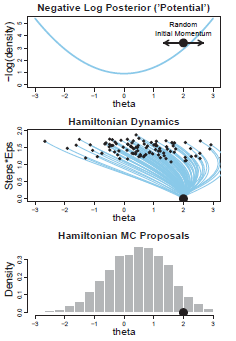
\includegraphics[scale=0.85]{Figures/Hamiltonian.png}
  \vspace{-14pt}
  \caption{Hamiltonian MCMC}
    \label{fig:Hamiltonian}
 \vspace{-16 pt}
\end{wrapfigure}

The \textit{rstanarm} package utilizes the implementation of Hamiltonian Monte Carlo
in \textit{Stan}, which is orders of magnitude more efficient than existing 
Markov Chain Monte Carlo (MCMC) algorithms for complex hierarchical models. Figure 
\ref{fig:Hamiltonian} reproduces Fig 14 in Kruschke \cite{Kruschke_Book_2014} to illustrate how 
\textit{Stan's} Hamiltonian algorithm achieves greater efficiency by using momentum to 
determine the next proposed draw from the posterior distribution. The current proposal's 
higher momentum (black dot) is indicated in the top panel. The middle panel illustrates how their 
momentum along with the gradient steers random samples to the mode of the posterior distribution (shown in lower 
panel) with the correct probability. 

Efficiency is critical during the sequential process of fitting intricate multilevel models to 
Big Data  and testing them, which can be cumbersome and slow even for sophisticated data scientists. 
Typically scientists have to explore and compare different 
angles and approaches to modeling large electronic data sets.  
Researchers need to update and tweak their models to make them more realistic, to 
incorporate knowledge about the subject matter, to fit the data better or 
to facilitate convergence of the algorithm. Other software, such as
WinBUGS and \textit{JAGS}, is not nearly efficient enough for complicated hierarchical models 
and / or large data sets. The challenges of fast 
and flexible computational implementation such limit the model sophistication 
(see letter by Dr. Kheterpal and Dutton). Researchers cannot fit multilevel 
models which reflect the actual hierarchical structure of clinical care delivered, 
(see letter by Dr. Sacks). Multilevel hierarchical models can compromise 
transparency with lengthy complicated programming code, making the process 
error prone (see letter of support by Dr. Pace). \textit{rstanarm's} simple 
yet flexible function calls facilitate dynamic model building and updating, 
and allows the fitting and testing of advanced models even for larger 
datasets. \textit{rstanarm} allows researchers to fit the model they 
believe to best reflect the clinical question they are investigating with EHR.

\subsection*{Improve tools for graphical exploration of hierarchical models and MCMC output}

\begin{wrapfigure}{l}{.6\textwidth}
  \vspace{-10pt}
 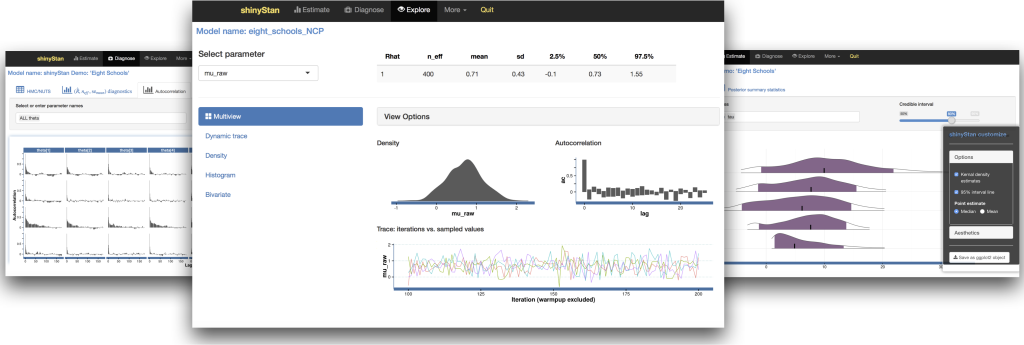
\includegraphics[scale=1.2]{Figures/shinystan.png}
  \vspace{-12pt}
  \caption{\textit{shinystan} interface}
    \label{fig:shinystan}
 \vspace{- 14pt}
\end{wrapfigure}

There is currently a dearth of tools to explore the enormous data stream 
generated by MCMC simulations in order to explore and troubleshoot the output of hierarchical models. 
\textit{shinystan} has started to fill this void and provide new visual methods to explore the output 
of sophisticated models, accelerate their development, reduce modeling errors and support inference. 
The interactive user interface \ref{fig:shinystan} of \textit{shinystan} 
provides powerful and easily accessible tools for posterior predictive checks 
of how well the model fits observed data. If a hierarchical 
model fails to converge, ascertaining why is crucial to troubleshooting. \textit{shinystan} 
is already unmatched in combining ease of interactive graphical exploration 
with sophisticated graphical rendering to explore visually and parameter 
specific co-linearity, autocorrelation, tree depth of Hamiltonian Monte 
Carlo algorithms and many other convergence diagnostics. We will not only 
further develop \textit{shinystan} to make it more robust and scale it to work 
faster for larger data sets. We will also develop novel graphical 
methods to assess model convergence and develop algorithms to 
troubleshoot model convergence with a special focus on hierarchical modeling.

\subsection*{Heterogeneous and incomplete clinical data may limit prediction and implementation.}
Variables with strong predictive power may not be recorded for all patients 
or may be missing for the time window needed for prediction, which is a critical limitation 
in the development of prediction algorithms and implementation of the 
therapeutic interventions (see letter of support by Dr. Mirhaji). 
Yet, incomplete data are the hallmark of EMRs. 
Likelihood-based mixed effects models for incomplete data give valid estimates 
\textit{if and only if } the missingness mechanism is ignorabe, which is to say that the parameters 
for the missing data mechanism are indpenent from the parameters in the main model for the 
outcome, and the data are either missing at random (MAR) or Missing Completely At Random 
(MCAR) \cite{Rubin1976}. Indeed, this is an unreasonable assumption for EMRs. In our example, only 
significant respiratory co-morbidity and symptoms will prompt physicians to request arterial blood gases (ABG). Trying to 
impute missing ABG data using multiple imputation would  hence lead to biased 
imputations as the ABG data will not be missing at random. Imputation using 
auxiliary data can overcome this limitation, as outlined below.

\subsection*{Auxiliary data can be used to impute incomplete medical records.} 

\begin{wrapfigure}{l}{10cm} 
 \vspace{-25pt}
 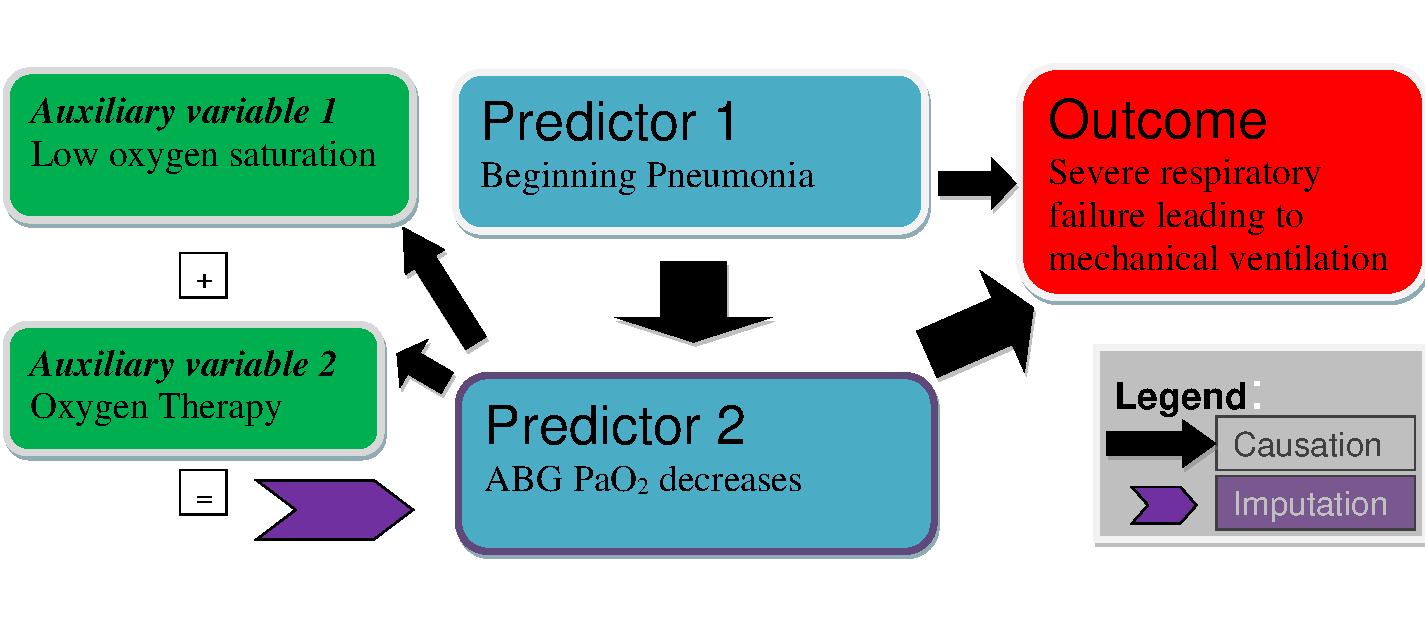
\includegraphics[scale=0.4]{Figures/Bayesian_imputation.pdf}
    \vspace{-20pt}
  \caption{Auxilliary data to impute missing information}
   \vspace{-15pt}
   \label{fig:Imputation_fig}
\end{wrapfigure}

Auxiliary data are additional information available in the form of variables known 
to be correlated with the missing data of interest 
\cite{Hall_25389642,Daniels24571539}. Figure \ref{fig:Imputation_fig} 
illustrates how we can impute incomplete data from auxiliary information 
\cite{Ibrahim2001auxilliaryImputaton,Schomaker23873614}. We know pneumonia 
impairs oxygenation, by causing respiratory failure, for example. If 
arterial $PaO_2$ (oxygen tension) is missing because arterial blood 
gases (ABG) have not been obtained, we can impute the incomplete data 
from oxygen therapy and/or peripheral oxygen saturation\cite{Hall_25389642}. 
This approach avoids the perils associated with missing at random (MAR) 
assumptions, when fitting a non-ignorable missingness model \cite{Wang_20029935}. 
Adding auxiliary variables not included in the main model for multiple imputation, 
in other words using additional information that is correlated with the missing 
outcome is an emerging approach to help correct bias 
\cite{Meng1994, Collins_11778676, Rubin1996}, often relying on 
Bayesian methods \cite{Daniels2008, Schafer1997}; joint hierarchical 
modeling, including auxiliary data to impute incomplete patient records, 
will improve the prediction model and facilitate the implementation of the 
prediction algorithm \cite{Hall_25389642}. Using auxilliary data to complete 
missing information is novel in data driven outcomes research and our 
software, \textit{rstanarm} and \textit{mi}, will disseminate this promising approach. 

\part*{Approach}

We propose to develop two accessible software packages, (\textit{rstanarm} 
and \textit{shinystan}), for the programming language and software environment 
\textit{R} to integrate incomplete information with hierarchical modeling for 
data driven outcomes research. These software products will make 
multidimensional statistical and computational methods for 
analyzing, inspecting, displaying, representing, parsing, and 
searching high-dimensional data more accessible to 
data scientists. We will also promote and disseminate these more realistic 
hierarchical modeling approaches through presentations, graduate teaching, 
workshops, online tutorials, books, YouTube videos and other publications.

We will develop our software further into solid, reliable, tested software packages. 
Both packages will serve as extension to the \textit{rstan} package we developed, 
which enables the most common applied regression models to be estimated using 
novel Hamiltonian Monte Carlo algorithms. All of these R packages are available to 
researchers and via the CRAN software repository. 

This project (software development and dissemination) will be guided by 
our multidisciplinary project team. The team will conduct its work through 
regularly scheduled weekly meetings and collaborate online via 
Github \cite{Chacon2009ProGit}, Google Hangouts, and email. 

\section*{Preliminary work}

\subsection*{Prior work in statistical software development and data driven outcomes research} 
Dr. Andreae published several meta-analyses and synthesized the evidence 
from clinical trials by pooling aggregate and individual patient data, when 
published results were insufficient for classical meta-analysis 
\cite{AndreaeJohnsonAbstract2013, Andreae2013, Andreae2015, Carter2015, Atchabahian2015}. Dr. Andreae, Hall, Goodrich and 
collaborators used the software \textit{rstanarm} and \textit{shinystan} to build a multilevel 
hierarchical model to investigate health care disparities and quality of 
anesthesia delivery in the large National Clinical Outcomes Registry maintained 
by the American Society of Anesthesiology \cite{AndreaeWhite2015}. Dr. Goodrich 
build \textit{mi}, a software package for the programming language and 
software environment R to impute missing data \cite{miCRAN}. Drs. Goodrich 
and Gelman developed along with other colleagues several widely cited and used software packages 
including the probabilistic programming language \textit{Stan}\cite{Stan_Software_2014}, 
which serves as the basis for the proposed work. Dr. Hall also published on missing data 
imputation \cite{Hall2009a, Wang_20029935, Wang_20029935} and is nationally 
recognized for the development and application of change point models in 
epidemiology and surveillance 
\cite{Hall2000, Hall2001, Hall2003bayesian, Hall2009, Hall2015}. 
More recently, Dr. Hall played a major role as the lead statistician 
for the World Trade Center (WTC) Health Program at the Fire Department 
of the City of New York, supervising data analyses based on medical 
records \cite{Aldrich2010, Hall2015, Zeig-Owens2011}.  
Dr. Gong's ongoing NIH funded trial to predict and improve 
respiratory outcomes after intubation based on real time 
electronic medical records is just one of many examples of her 
leading role in applied data driven outcomes research 
\cite{Gong2005, Gong2010, Gajic2011, Yu_24970344, Kor2014}. 
Dr. Gelman is internationally recognized as a leader in Bayesian and hierarchical 
modeling and data imputation 
\cite{Gelman1998notasked, Gelman2001imputation, Hoffman2014, Gelman-Hill_2014}. 
Dr. Gelman, co-investigator on this grant, and his collaborators has been laying the 
theoretical ground work for the development of the cutting-edge Hamiltonian 
Monte Carlo algorithms \cite{Hoffman2014,Stan_Software_2014} 
that are at the basis of \textit{Stan}, the engine 
under the hood of our user oriented software package \textit{rstanarm}, 
this project proposes to develop. His team includes Dr. Betancourt, 
consultant on this grant with his special expertise on the differential 
geometry of the underlying Hamiltonian Monte Carlo algorithm
motivating automated tuning heuristics and certain optimality criteria 
\cite{BetancourtGeometry2016}, which will play a 
critical part in our programming of the \textit{Stan} model library 
which \textit{rstanarm} will call on and in the tools for graphical exploration
we propose to implement in \textit{shinystan}.

\subsection*{The trajectory leading to the development of the prototype software} 

\begin{wrapfigure}{l}{0.6\textwidth} %this figure will be at the right
    \centering
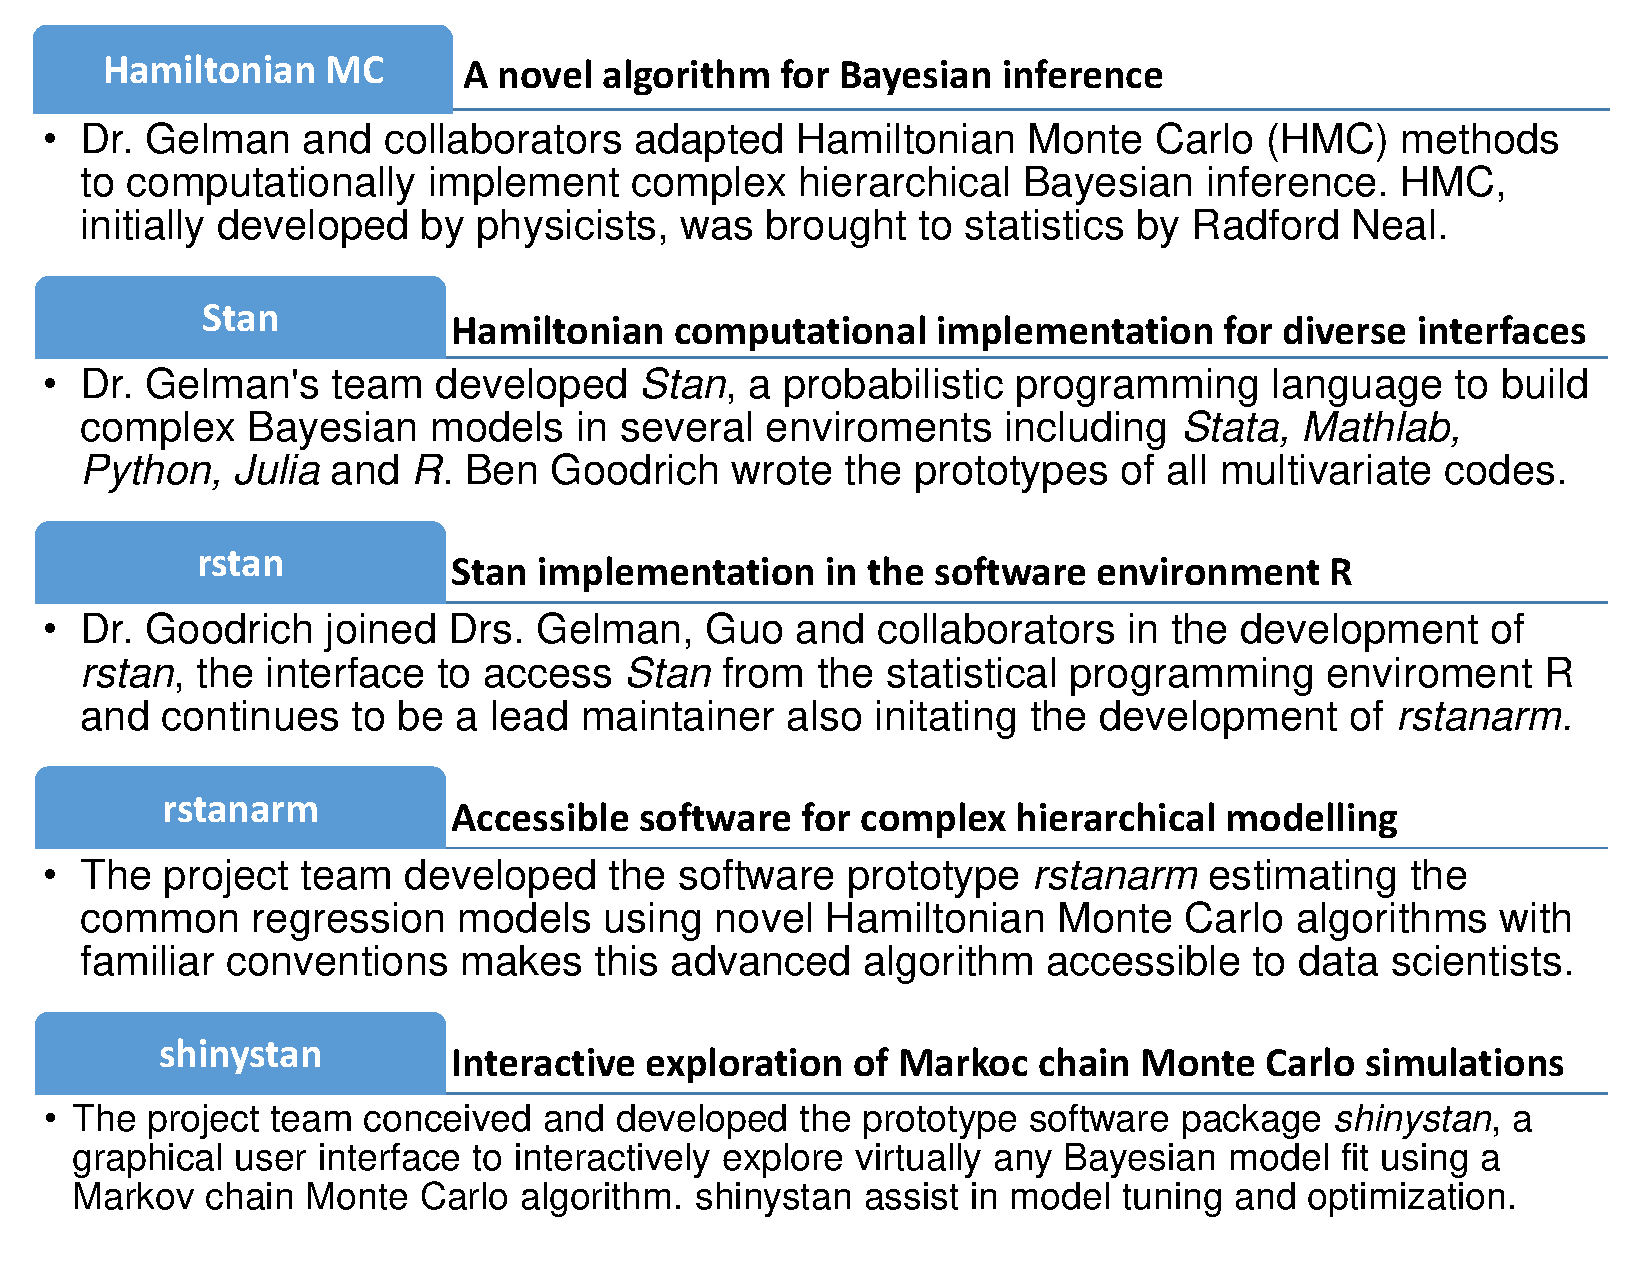
\includegraphics[width=0.6\textwidth]{Figures/SoftwareTrajectory.pdf}
\end{wrapfigure}

Dr. Goodrich, Andreae, and their collaborators worked together on the software packages 
\textit{shinystan} and \textit{rstanarm}, which are extensions to the \textit{rstan} package 
that enables some of the most common applied regression models to be estimated using Hamiltonian Monte Carlo. 
The National Institute of Health, the Center for Disease Control and the National Science Foundation, 
(NIH: 5R01GM074806, 5KL2TR001071, UH2-HL125119,  CDC: U01 OH010711-01 and NSF: SES-1205516) were among the many 
federal institutions funding our team's prior software \cite{Stan-manual:2015} development and their application 
to cutting=edge biomedical data driven outcomes research. The proposed work is hence a direct continuation of the 
above described preliminary work of developing and implementing novel ground breaking algorithms for hierarchical 
modeling of fine grained correlated data and their biomedical applications. In the graphic to the left above, we 
outline the trajectory that led to the current project proposal.


\section*{Project scope and goals }

The project proposes to develop two accessible software packages for the programming language and software environment \textit{R} 
to integrate incomplete information with hierarchical modeling for data driven outcomes research. We propose to develop two applications.

\subsection*{rstanarm for accessible multilevel hierarchical modeling}
The first proposed software package \textit{rstanarm} should allow data scientists to specify the most common applied regression models 
and hierarchical models and estimate them via the Hamiltonian Monte Carlo (HMC) algorithm implemented in \textit{Stan} without (a) 
the need to understand the underlying intricacies (e.g., auxiliary parameterization) normally required to optimize convergence and 
without (b) the need to build large convoluted contrast matrices  or keep track of level indexing. Using the same familiar notation for 
model formulation as other popular software packages for linear and mixed modeling in \textit{R} like \textit{lme4} \cite{lme4}, will 
make model building easy for novice \textit{rstanarm} users. 

\subsection*{shinystan for interactive graphical exploration and diagnosis of MCMC simulations}  
The second package, \textit{shinystan}, is a graphical user interface for interactively exploring any model estimated by MCMC. As a 
package for \textit{R}, \textit{shinystan}  provides multidimensional statistical, graphical and computational tools for any analyzing,
inspecting, displaying, representing, parsing, and searching high-dimensional MCMC output, but is optimized for HMC. By using a web-based 
interactive intuitive user interface \textit{shinystan} is user-friendly and requires minimal training for novices.

\subsection*{rstanarm and shinystan are available on the \textit{R} software repository CRAN}
Both \textit{rstanarm} \cite{rstanarm} and \textit{shinystan} \cite{shinystan, Team2015} are available on the \textit{R} software 
repository CRAN. The project proposes to further develop these two prototypes \textit{rstanarm} and \textit{shinystan} into solid, 
reliable, tested R packages and to disseminate their use. Both packages will serve as extensions to the \textit{rstan} package 
(we developed), which enables the most common applied regression models to be estimated using novel Hamiltonian Monte Carlo algorithms. 
The final product packages will be available to researchers and the general public via the free software repository CRAN. 

\section*{Software Specification}

\subsection*{rstanarm}
The software package \href{https://github.com/stan-dev/rstanarm}{\textit{rstanarm}}
will enable the estimation of advanced applied general linear regression models using 
the existing probabilistic programming language \textit{Stan}. 
\textit{rstanarm} implements full Bayesian statistical inference;  
however, \textit{rstanarm} allows users to specify their 
hierarchical models using the simplified syntax already commonly 
used in standard software packages like \textit{lme4} in the statistical 
software environment \textit{R}. 

\subsubsection*{rstanarm allows simple specification for multi-level hierarchical models}

Data scientists familiar with the widely used statistical software environment R will 
find \textit{rstanarm} intuitive, because models are specified using the familiar 
standard R modeling syntax to describe the mean structure of mixed models. 
For example, \textit{rstanarm} uses the same a two-sided 
linear formula syntax describing both the common and group-specific parameters that was 
invented by \textit{lme4},  e.g.:

\begin{wrapfigure}{l}{.2\textwidth}
\vspace{-30pt}
\begin{equation}
y \sim x1 +(x2|g)
\end{equation}
\vspace{-40pt}
\end{wrapfigure}

where the dependent response variable $y$ is on the left of a Tilde ($\sim$) operator; 
the independent terms, $x_1, x_2...$ are on the right and separated by the $+$ 
operator. Group-specific terms are distinguished by vertical bars $|$ 
separating expressions for design matrices from grouping factors. Clinical data 
scientist can therefore take advantage of the more efficient HMC algorithms implemented in \textit{Stan}, 
without knowing the underlying programming language or the auxiliary reparametrizations that 
increase the efficiency of the Markov chains, which we discuss further below.

\subsubsection*{A suite of pre-compiled \textit{Stan} programs allows for a simple call to sophisticated modeling functions}

\textit{rstanarm} already implements many generalized linear 
models with and without group-specific terms. We wrote and optimized several models 
in the probabilistic programming language \textit{Stan} that are
pre-compiled in \textit{rstanarm}. Users can now build hierarchical models via simple high-level functions, as detailed below.

\begin{wraptable}{l}{0.6\textwidth}
\footnotesize
\begin{tabular}{@{}
>{\columncolor[HTML]{EFEFEF}}l l@{}}
\toprule
\textbf{Function Call} & \textbf{Underlying process}                        \\ \midrule
stan\_aov               & User interface for simplified model specification  \\
stan\_lm               & Parsing linear model specification \\
stan\_lm.fit           & Workhorse function to call pre-comiled \textit{Stan} model  \\
lm.stan                & Pre-compiled optimized model written in \textit{Stan}                   \\ \bottomrule
\end{tabular}
\label{ProcessTable}
\end{wraptable}

To take an ANOVA model as an example, the wrapper function $stan\_aov$ parses the 
model specification and hands the data and prior specification to $stan\_lm$ and 
then to a lower-level workhorse function, $stan\_lm.fit$, which in turn 
calls the pre-compiled and optimized \textit{Stan} model specified in 
$lm.stan$. The the Hamiltonian Monte Carlo output is returned in reverse order
through these functions to the data scientist in a list that is convenient 
for analysis, plotting, and other post-estimation functions.

The $stan\_lm$, $stan\_glm$ and $stan\_glmer$ functions are similar in syntax to the R functions $glm$ 
and $glmer$ but rather than performing maximum likelihood estimation of classical generalized linear models, 
\textit{rstanarm} emphasizes full Bayesian estimation via Hamiltonian Monte Carlo. If "weakly informative" 
priors are chosen in simple models, the posterior means will tend to be very similar to classical frequentist point 
estimates \cite{Gelman-Hill_2014}. However, \textit{rstanarm} uses the same user-friendly interface to estimate 
sophisticated hierarchical models that are too complicated for classical frequentist inference.

\subsubsection*{Prior specification for regularization or to incorporate external information}

Priors \textit{can} incorporate subjective beliefs or existing information 
about a parameter,  which we discussed in more detail under significance \
\cite{carlin1997bayes}. 
Priors can be used to regularize classical models \cite{gelman2008weakly}. 
Bayesian models require priors and \textit{rstanarm} by default usually
adds independent weakly informative priors on the coefficients of generalized linear models, 
but more informative priors can be specified by the user. Especially in hierarchical modeling, 
regularization with priors can help convergence and improve inferences 
\cite{Gelman-Hill_2014}. In \textit{rstanarm}, specification of the prior 
can such be left to the default implementation or the user can choose from 
a broad array of distribution, (e.g., for the intercept one might choose the 
Student t distribution, which approaches the normal distribution as the 
degrees of freedom approach infinity and as the degrees of freedom are 
one or the Cauchy distribution, leaving the user the option of robust 
priors to allow for outliers to achieve more robust inference). 

\subsubsection*{Further hardening, expansion and integration of \textit{rstanarm}}
While \textit{rstanarm} delivers some functionality for data scientist and is already available from 
\href{https://cran.rstudio.com/web/packages/rstanarm/}{CRAN}, much of this project will be devoted to hardening existing functionality, 
expanding functionality, and integrating functionality from other R packages. We need to incorporate user feedback, weed out 
possible bugs, and include many more functions and advanced models, such as change-point models \cite{Hall2000}. Specifically, 
we want to work on a more seamless integration with our \textit{R} package for multiple imputation of missing data 
\href{https://cran.r-project.org/web/packages/mi/index.html}{\textit{mi}}.

\subsection*{shinystan}
We propose to develop \href{http://andrewgelman.com/2015/03/02/introducing-shinystan/}
{\textit{shinystan}} \cite{GabryISCB2015,shinystan} as a the 
graphical user interface for interactively 
exploring virtually any Bayesian model output but optimized for \textit{Stan}. 

\subsubsection*{Goal: interactive intuitive graphical exploration of MCMC output} 
To extract the results from objects representing model fits, data scientist can 
use generic extractor functions such as print() and coef(), but often lack a suitable 
method for extracting an interesting result of the model fit and have to resort to 
writing tedious customized code. Important model diagnostics 
(e.g., influence() to assess  homoscedastic residual errors) are not 
developed even for classical multi-level models \cite{Galecki2013linear}, 
and data scientists certainly lack tools for interactive intuitive graphical 
exploration of MCMC output.

\subsubsection*{Implementation}
We will further implement \textit{shinystan}
in \textit{Shiny}, an R package for interactive 
web applications. The graphical rendering of the plots in \textit{shinystan} 
utilizes the superb graphical package \textit{ggplot} by Hackley Wickham. 
Many of our new graphical functions of \textit{shinystan} will eventually be 
integrated directly into \textit{rstan} to allow users to integrate the graphical 
and numerical output of \textit{shinystan} directly into reports generated with 
markdown in R through the \textit{knitr} package.

\subsubsection*{Model checking}
shinystan will facilitate many diagnostics to optimize model convergence, explore unexpected parameter 
correlations, and assess the correctness of the model specification. Here we will delineate two examples.
\begin{enumerate}
\item (a) residual diagnostics, e.g., for continuous covariates, a scatterplot of the residuals against the values of the covariate
 
\item (b) influence diagnostics
\end{enumerate}

\subsubsection*{Automation of meta-data extraction and management in \textit{shinystan}}
The automation of many data exploration processes saves time, but implies the extraction of the meta-information about the model and 
its parameters as detailed in Table \ref{ObjectCharactersitics}. Data scientist working with the raw draws from the MCMC output 
have to extract, manage and program a plethora of details to explore higher level structure and statistics of their output. 

\begin{wraptable}{l}{0.7\textwidth}
\footnotesize
\begin{tabular}{@{}
>{\columncolor[HTML]{EFEFEF}}l l@{}}
\toprule
\textbf{Object} & \textbf{Increasingly informative object characteristics} \\ \midrule
MCMC & raw data from Markov chain Monte Carlo chains \\ \midrule
rstan & structured embedded model information (\textit{Stan} code, parameter names...) \\ \midrule
rstanarm & accessible aggregate derived statistics (coefficients, SE, fitted, residuals) \\ \midrule
shinystan & detailed user-friendly model meta-data, posterior predictive draws... \\ \bottomrule
\end{tabular}
\caption{Progressive enrichment of object characteristics in \textit{shinystan} }
\label{ObjectCharactersitics}
\end{wraptable}

As we move from the MCMC output (raw draws from posterior
distributions) to the user-facing output object structures become richer with model-specific 
information (e.g., \textit{Stan} code). The user-friendly \textit{rstanarm} 
package contains even more accessible information that is derived from the original function call. 
Finally, the interactive web based tool \textit{shinystan} extracts and processes much more meta-data to 
facilitate interactive and intuitive visual exploration and troubleshooting.

\subsubsection*{Affordances: designing intuitive user interfaces}
We will place special emphasis on the concept of affordance in our "intuitive" 
design of the \textit{shinystan} graphical user interfaces, e.g., in employing 
strong visual clues, provide clickable buttons and tabs, sliders, and other 
hands on interactive controls \cite{NormanAffordances1999}. Active exploration 
by \textit{shinystan} users will reveal nested and sequential affordances, for 
example, print options appear only in context, say when the cursor moves over 
the output button of a graphic, avoiding visual clutter on the screen with 
irrelevant information \cite{Mcgrenere2000affordances}. We will rely on user 
feedback to optimize the practical utility of \textit{shinystan's} implementation 
and user interface.

\subsubsection*{Improving and hardening \textit{shinystan}}
Although already available on 
\href{https://cran.r-project.org/web/packages/shinystan/index.html}{CRAN} 
as a functional \href{https://www.youtube.com/watch?v=X31xqNHcvQs}{package},
\textit{shinystan} will need to undergo considerable improvements of the 
interface and under the hood during this project. Posterior predictive 
checking is one area where the need for additional options and functionality. 
We also want to expand the existing collaborative model sharing via the internet.

\section*{Collaborative software development and computer resources}
\subsection*{Best practices and proven methods for software design, construction, and implementation}
We will follow accepted best practices, proven methods, and industry standards for software design, construction and implementation.
For example the rules of clarity, composition, separation, simplicity, parsimony, transparency, etc. as detailed by 
Raymond \cite{Raymond2003art}, as we did in building \textit{rstan} and \textit{Stan}. We will pay special attention to modularity 
and function routines in the design of our software packages and on the integration with existing subroutines already written in the 
parent software suites \textit{Stan} and \textit{rstan}. 

\subsubsection*{Collaborative code development using online repositories }
The source code of \textit{rstanarm} and \textit{shinystan} are managed through the Git version control system 
\cite{Chacon2009ProGit} via the online software repository \href{https://github.com/}{Github} for integrated issue tracking, 
progress milestones, and code history tracking \cite{loeliger2012version}. We will use the Git process \cite{Driessen2010successful}, 
as we did sucessfully for the development of \textit{Stan} \cite{Stan-manual:2015}. This  process is based on collaborative code review, 
where new features or functions are developed creating a branch; proposed changes and additions are discussed following a pull request on 
Github. The ability to write to the repository is restricted to the core team, while any user can propose patches to address software 
bugs or suggest improvements. Further commits are commonly added after substantial feedback and testing before merging the branch.  
On Github, altered syntax is highlighted and changes are transparent and revertible, making collaborative software development easier. 
Github's distributed structure implies that everybody cloning the repository generates a backup. We prototype and test additional 
functions and features before inserting them in any package update. All of our code is thoroughly tested.

\subsubsection*{Communication}
The development, extension, testing and maintenance of our packages is a collaborative effort by our multidisciplinary team with 
communication and input taking place in several venues. Public user groups and discussion are archived and freely accessible. 
Confidential deliberations, (e.g., regarding grant related matters), are held in private restricted groups. We will hold weekly video 
conferences to prioritize issues and discuss progress.

\subsection*{Computer resources and data security}
\subsubsection*{Montefiore medical and Columbia University computer cluster access}
Montefiore Medical and Columbia University will provide the computer cluster access required for the computationally more intensive 
models and provider server space to house the software and webpages. We will run models in our statistical software packages in parallel 
for statistical inferences of large hierarchical clinical data sets. Clinical Research Informatics at Montefiore will provide scale-able 
remote access via a secure virtual private network to up to 32 Xenon Intel processors in parallel on a windows virtual machine with up to 
128 GB RAM to meet the variable needs of the project throughout the course of the grant. 

\subsubsection*{Data security and confidentiality}
As also discussed under human subject protection and in resources and in the letter of support by Dr. Mirhaji, some of the data sets to 
be used for this project cannot be completely de-identified, but are 'limited data sets', because they still contain some patient 
identifiers (e.g., age in years or zip code) and as such are covered under HIPPA. Hence, the computer clusters housing the data and where 
we run the analysis on, have to be compliant with the Health Insurance Portability and Accountability Act (HIPPA. Clinical Research 
Informatics at Montefiore will house any data set falling under the Health Insurance Portability and Accountability Act (HIPPA) and 
guarantee compliance with relevant federal data safety and privacy regulations. 

\section*{Dissemination and unimpeded utilization of the products of this project}
The goal of this project is to encourage widespread adoption of cutting edge 
hierarchical modeling for data driven outcomes research by clinical scientists and to support the use and re-purposing of our 
open-source applications. As also detailed in the data sharing plan, to facilitate the widest 
possible uninhibited unimpeded utilization, our software will be 
licensed under the General Public License and will be available on 
the online repository CRAN. The benefits  are that our products 
\textit{rstanarm} and \textit{shinystan}: 
 
1) will be freely available to researchers and the general public, including for commercial use; 

2) shall remain freely available to the public;

3) may be freely extended, customized, and incorporated into the other tools that also are licensed under the same terms; 

4) can be maintained if the original developers are no longer able to; 

5) can be enhanced based on user-provided feedback for bug-fixes, examples, and enhancements.

The software developed for this grant will hence all be incorporated into the public repository CRAN, 
the Comprehensive R Archive Network of the open-source R Project for Statistical Computing. Our source code and documentation 
will be distributed under the least restrictive open-source licensing terms possible: R's licensing is \textit{copyleft} under the 
GNU General Public License. \textit{Copyleft} refers to licensing arrangement that allow for the software can be used, modified and/or 
distributed freely on condition that anything derived is bound by the same condition. 

\subsection*{Dissemination}
\subsubsection*{Prior team experience and exposure in statistical and quantitative teaching and dissemination}
Our project team have ample experience in teaching, publishing and promoting software and quantitative methods and skills in the project 
team, including faculty in graduate programs focused on teaching quantitative skills to social science and biomedical audiences. 
Our workshops on statistical and research methods are sought after and invited to national and international statistical and biomedical 
meetings; our team presented workshops at a wide spectrum of scientific and statistical meetings ranging from clinically oriented 
conferences like the Annual meeting of the American Society of Anesthesiologists to machine learning venues like the Annual Conference 
on Neural Information Processing Systems (NIPS). Presentations  and products by our team have been featured on YouTube and blogs.   

\subsubsection*{Books, tutorials, workshops lectures and outreach}
Throughout the duration of the project we will disseminate the software packages in tutorials, workshops, lectures, books and other forms 
of outreach. In particular, we will offer hands on workshops in small groups to multipliers based on our applied practical use cases at 
international conferences as outlined also in the budget justification. These will be interlinked and supported by online material, for 
example YouTube videos \href{https://www.youtube.com/watch?v=pWow8Qe1snQ}{promoting} or 
\href{https://www.youtube.com/watch?v=pHsuIaPbNbY}{explaining and motivating} the algorithms underlying \textit{Stan}. We will make 
detailed \href{http://mc-stan.org/documentation/}{technical} and practical tutorials and 
\href{https://cran.r-project.org/web/packages/rstanarm/vignettes/aov.html}{vignettes} available online, interspersing code, graphics 
and detailed step by step explanations using \textit{R's}  \href{http://rmarkdown.rstudio.com/}{R Markdown \- Dynamic Documents for R}, 
blogs, for example our \href{http://andrewgelman.com/}{blog} on Statistical Modeling, Causal Inference, and Social Science and 
textbooks \cite{Gelman-Hill_2014}. 

\subsubsection*{Mechanisms for incorporating feedback and user reported corrections into the software.}

We already have very active \href{https://groups.google.com/forum/#!forum/stan-users} {user groups} around \textit{Stan} and 
\textit{rstan}  with frequent online and face-to-face \href{http://www.meetup.com/bda-group/}{meetings}. We will incoporate more of
\textit{rstanarm} and \textit{shinystan} in the future to to discuss implementation issues, engage advanced users in the development of 
our packages and/or in designing courses around our models and software, but in particular to solicit their feedback. The user 
forums have served also to assist novices in implementing their models in our software.
Like our existing \href{https://github.com/stan-dev/example-models/wiki}{Wiki} on Github for \textit{Stan}, we will 
take full advantage of the functionality of GitHub for engaging users in collaborative software development \cite{loeliger2012version}, 
including further develop our \textit{rstanarm} and \textit{shinystan} 
\href{https://github.com/stan-dev/rstanarm/wiki}{Wikis} and discuss \href{https://github.com/stan-dev/rstanarm/issues}{issues} with users.

\section*{Timeline and potential problems}

\begin{wrapfigure}{l}{0.7\textwidth} %this figure will be at the right
    \centering
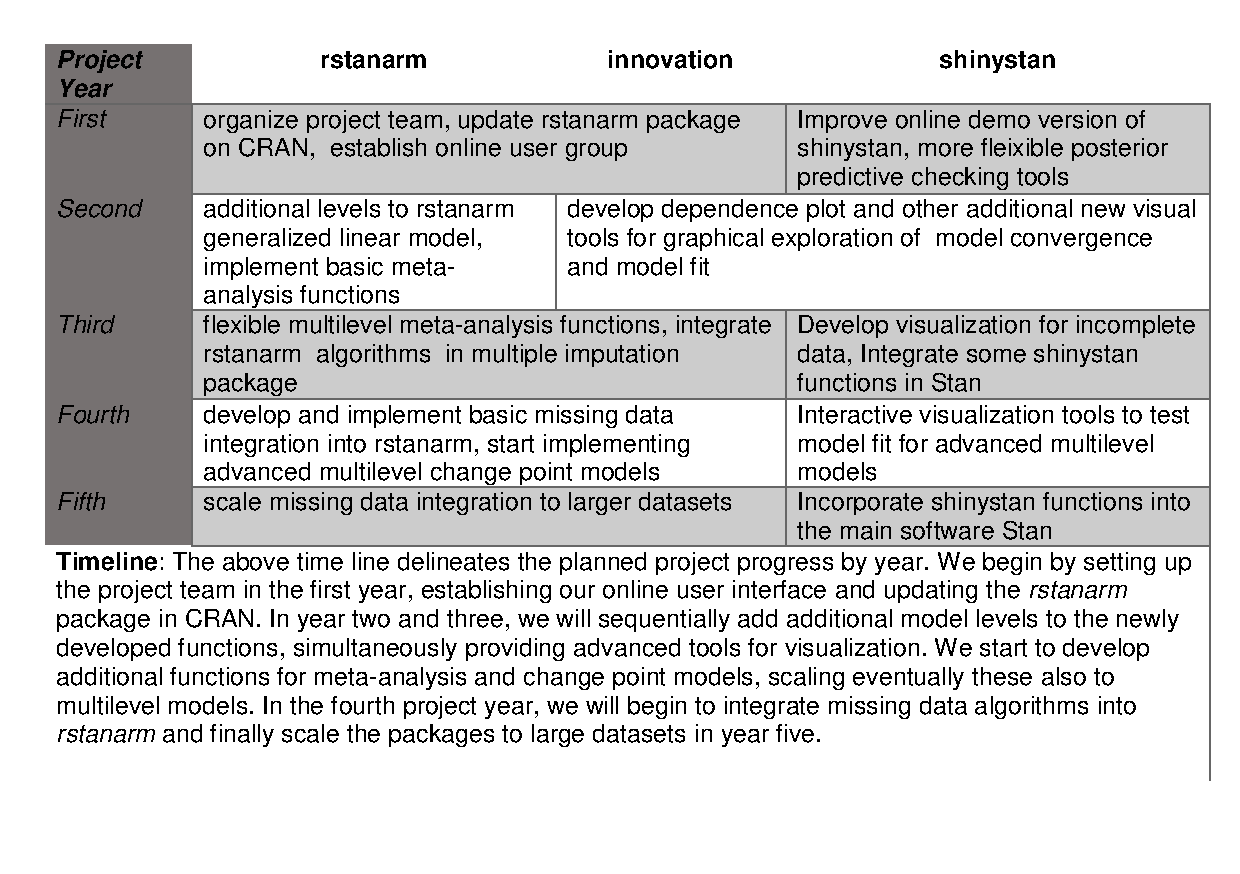
\includegraphics[width=0.7\textwidth]{Figures/Timeline.pdf}
\end{wrapfigure}

The adjacent time line delineates the planned project progress by year. We begin by setting up the project team in the first year, 
establishing our online user interface and updating the \textit{rstanarm} package in CRAN. In year two and three, we will sequentially 
add additional models and provide advanced tools for visualization. We start to develop additional functions for meta-analysis and 
change-point models, scaling eventually these also to multilevel models. In the fourth project year, we will begin to integrate 
missing data algorithms into \textit{rstanarm} and finally scale the packages to large datasets in year five.

Some colleagues are reluctant to make powerful statistical tools accessible to the novice users that do not understand them. We counter 
however that the simplicity of the \textit{rstanarm} syntax will allow novice users to learn to specify more realistic models by 
making the underlying hierarchical model structure more transparent.  \textit{rstanarm} will also allow outcomes research to be 
more transparent and reproducible. Also \textit{shinystan} will contribute to the ease with which advanced hierarchical models and MCMC 
results can be shared, questioned, and discussed.
 
%----------------------------------------------------------------------------------------
%	BIBLIOGRAPHY
%----------------------------------------------------------------------------------------

\newpage

% \nobibliography{K01_bibliography_24Feb15} % to not print a bibiography at the end.
\bibliography{Bibliography/bibliographyBD2K} % the file name cannot contain spaces
\bibliographystyle{Bibliography/nihunsrt} % Use the custom nihunsrt bibliography style included with the template

%----------------------------------------------------------------------------------------

\end{document}
